\clearpage
\item \points{15} {\bf Logistic Regression: Training stability}

In this problem, we will be delving deeper into the workings of logistic
regression. The goal of this problem is to help you develop your skills
debugging machine learning algorithms (which can be very different from
debugging software in general).

We have provided an implementation of logistic regression in
\texttt{src/p01\_lr.py}, and two labeled datasets $A$ and $B$ in
\texttt{data/ds1\_a.txt} and \texttt{data/ds1\_b.txt}.

Please do not modify the code for the logistic regression training algorithm
for this problem. First, run the given logistic regression code to train two
different models on $A$ and $B$. You can run the code by simply executing 
\texttt{python p01\_lr.py} in the \texttt{src} directory.

\begin{enumerate}

  \item \subquestionpoints{2}
What is the most notable difference in training the logistic regression model
on datasets $A$ and $B$?

\ifnum\solutions=1 {
  \begin{answer}
the model can converge easily on Dataset A, while the model can hardly converge on Dataset B.
\end{answer}

} \fi


  \item \subquestionpoints{5}
Investigate why the training procedure behaves unexpectedly on dataset $B$, but
not on $A$. Provide hard evidence (in the form of math, code, plots, etc.) to
corroborate your hypothesis for the misbehavior. Remember, you should address
why your explanation does \emph{not} apply to $A$.

\textbf{Hint}: The issue is not a numerical rounding or over/underflow error.

\ifnum\solutions=1 {
  \begin{answer}
\begin{figure}[htb]
    \begin{subfigure}{0.5\linewidth}
        \centering
        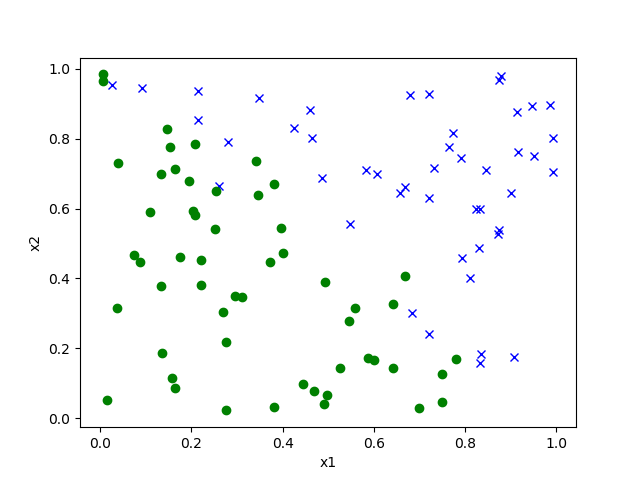
\includegraphics[width=\linewidth]{tex/a.png}
        \subcaption*{Dataset A}
    \end{subfigure}
    \begin{subfigure}{0.5\linewidth}
        \centering
        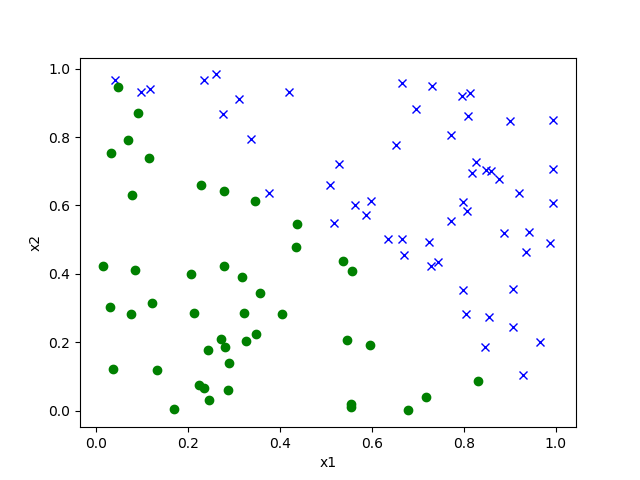
\includegraphics[width=\linewidth]{tex/b.png}
        \subcaption*{Dataset B}
    \end{subfigure}
    
\end{figure}
The dataset B is perfectly linear separable. In this case, when the logistic regression finds a decision boundary that can separate the dataset perfectly, the algorithm can decrease the negative log-likelihood function by multiplying the $\theta$ by a arbitrary number. However, multiplying the $\theta$ by a number doesn't change the decision boundary. Like the functional margin of SVM, we can make the $\theta$ arbitrarily large without really changing anything meaningful. 
Logistic regression can converge on the dataset A, because that dataset is not linearly separable.
\end{answer}

} \fi


  \item \subquestionpoints{5}
For each of these possible modifications, state whether or not it would lead to
the provided training algorithm converging on datasets such as $B$. Justify your
answers.
\begin{enumerate}
  \item Using a different constant learning rate.
  \item Decreasing the learning rate over time (e.g. scaling the initial
  learning rate by $1/t^2$, where $t$ is the number of gradient descent
  iterations thus far).
  \item Linear scaling of the input features.
  \item Adding a regularization term $\|\theta\|_2^2$ to the loss function.
  \item Adding zero-mean Gaussian noise to the training data or labels.
\end{enumerate}
 
\ifnum\solutions=1 {
  \begin{answer}\\
(i) No. The theta will still arbitrarily increase but in a slow speed.\\
(ii)Yes. This modification will make the learning rate decreasing very quickly in order to force the algorithm to stop updating the $\theta$.\\
(iii) No. The dataset will still be linear separable.\\
(iv) Yes. This will prevent $\theta$ to be arbitrarily large.\\
(v) No. Actually, the result depends on how much the noise is. It should be large enough to make the dataset not linearly separable. If the noise is small, the linear-separable-dataset problem is still not solved.
\end{answer}

} \fi

 
  
  \item \subquestionpoints{2}
Support vector machines (SVMs) are an alternative machine learning model that we discussed in class.
We have provided you an SVM implementation (using a radial basis function (RBF) kernel) within \texttt{src/svm.py} (You should not need to modify that code).

One important part of training an SVM parameterized by an RBF kernel is choosing an appropriate kernel radius.

Complete the \texttt{compute\_best\_svm\_radius} by writing code to compute the best SVM radius which maximizes accuracy on the validation dataset.

The provided code will use your \texttt{compute\_best\_svm\_radius} to compute and then write the best radius into \texttt{output/p06\_optimal\_radius}.

\ifnum\solutions=1 {
  \begin{answer}
The optimal SVM radius was 0.1. The accuracy on the test set is 0.9695
\end{answer}

} \fi



\end{enumerate}

\textbf{Hint:} Recall the distinction between functional margin and geometric
margin.
